% $Id: qcd-colliders.tex 528 2019-10-25 06:01:20Z smarzani $
%
% Introduction to QCD at colliders (not exactly clear what this means)
% ------------------------------------------------------------------------
\chapter{Introduction to QCD at Colliders}\label{chap:qcd-colliders}
Jet physics is QCD physics. Therefore, a solid and insightful
description of jets and their substructure relies on a deep understanding of the dynamics of strong interactions in collider experiments. 
%
QCD is an incredibly rich but, at the same time, rather complicated theory and building up a profound knowledge of its workings goes beyond the scope of this book. At the same time, some familiarity with perturbative calculations in quantum field theory is necessary in order to proceed with our discussion.
%
Therefore, in this chapter we recall the essential features of the theory of strong interactions that are needed in jet physics.
%
Because we aim to make this book accessible to both theorists and experimenters that want to move their first steps in jet substructure, we are going to take a rather phenomenological approach and we will try to supplement the lack of theoretical rigour with physical intuition. QCD itself helps us in this endeavour because the dynamics that characterises jet physics is often dominated by soft and collinear radiation, \ie emissions of partons that only carry a small fraction of the hard process energy or that are emitted at small angular distances. The structure of the theory greatly simplifies in this limit and many results can be interpreted using semi-classical arguments. The price we have to pay is that, if we want to achieve a reliable description of observables in the soft and collinear regions of phase-space, we have to go beyond standard perturbation theory and consider the summation of some contributions to all orders in perturbative expansion. 



\section{The theory of strong interactions}
Let us begin our discussion with a historical detour. 
%
The quest for a coherent description of strong interactions started in the 1960s and had the principal aim of understanding and classifying the plethora of new
particles produced at the first particle colliders. 
%
Indeed, as machines to accelerate and collide particles were becoming more powerful, many new strongly-interacting particles, collectively referred to as hadrons, were produced, leading to what was defined as a particle zoo. Some of these particles shared many similarities to the well-known protons, neutrons and pions and could therefore be interpreted as excited states of the formers. Other particles instead presented new and intriguing properties. 
%
A major breakthrough was realised with the \emph{quark model}.
%
This model successfully applied the formalism of group theory to describe the quantum numbers of the hadrons known at that time. It introduced fundamental constituents with fractional electric charge called quarks and described mesons and baryons in terms of the different combinations of these constituents. However, the model made no attempt to describe the dynamics of these constituents. 
%
The quark model led to another important discovery: the introduction of a new degree of freedom, which was termed colour. Its introduction was made necessary in order to recover the symmetry properties of the wave-function of some baryonic states such as the $\Delta^{++}$ or the $\Omega^-$.

Alongside hadron spectroscopy, scattering processes were used to study the structure of the hadrons. In this context, experiments where beams of electrons were scattered off protons played a particular important role, as they were used to probe the structure of the protons at increasingly short distances. 
%
The experiments in the deep-inelastic regime, where the target protons were destroyed by the high-momentum-transfer interaction with the electron, pointed to  peculiar results. The interaction was not between the electron and the proton as a whole, but rather with pointlike constituents of the proton, which behaved as almost-free particles. 
%
In order to explain these experimental data, the \emph{parton model} was introduce in the late Sixties.
 The basic assumption of this model is that in high-energy interactions, hadrons behave as made up of almost free constituents, the partons, which carry a fraction of the hadron momentum.
 Thus, the description of the hadron is given in terms of partonic
distributions that represent the probability of having a particular
parton which carries a fraction of the total hadron's momentum.

The quark model and the parton model aim to describe rather different physics: the former classifies the possible states of hadronic matter, while the latter applies if we want to describe how a hadron interacts at high energy. However, it is very suggestive that they both describe hadronic matter as made up of more elementary constituents. 
%
A successful theory of the strong force should be able to accommodate both models. Nowadays Quantum Chromo-Dynamics (QCD) is accepted as the theory of strong interactions.
It is a non-Abelian gauge theory and the symmetry group is the local version of the colour symmetry group SU(3). The theory describes the interaction between fermionic and bosonic fields
associated to quarks and gluons respectively (see for instance~\cite{Peskin:257493,Schwartz:2013pla,Collins:1350496,Ellis:1991qj,Campbell:2286381} and references therein).

The QCD Lagrangian
\begin{equation}\label{eq:qcd-lagrangian}
\mathcal{L}= -\frac{1}{4}F^A_{\mu\nu}F_A^{\mu\nu}+
\sum_\text{flavours}\bar{\psi}_a (i \gamma_\mu D^\mu-m)_{ab}\psi_b \,,
\end{equation}
where  $F^A_{\mu \nu}$ is
the gluon field strength, defined by:
\begin{equation}\label{eq:qcd-fs}
F_{\mu\nu}^A= \partial_\mu A_\nu^A - \partial_\nu A_\mu^A +
g_sf^{ABC}A_\mu^BA_\nu^C \,.
\end{equation}
and $D_\mu$ is the covariant derivative
\begin{equation}
\left( D_\mu\right)_{ab}=\partial_\mu \delta_{ab}- i g_s A_\mu^A t^A_{ab},
\end{equation}
where $t^A$ are the algebra generators.
In the above equations both lower-case and upper-case indices indicate refer to SU(3), the formers denote indices in the (anti)-fundamental representation, while the latter in the adjoint one. We note that a sum over quark flavours, namely up, down, charm, strange, top, and bottom is indicated. Strong interactions are completely blind to this quantum number and therefore the only distinction between different quark flavours in this context comes about only because of the mass. Note that the quark masses span several orders of magnitude and therefore the related phenomenology is extremely different!


\begin{figure}
\begin{center}
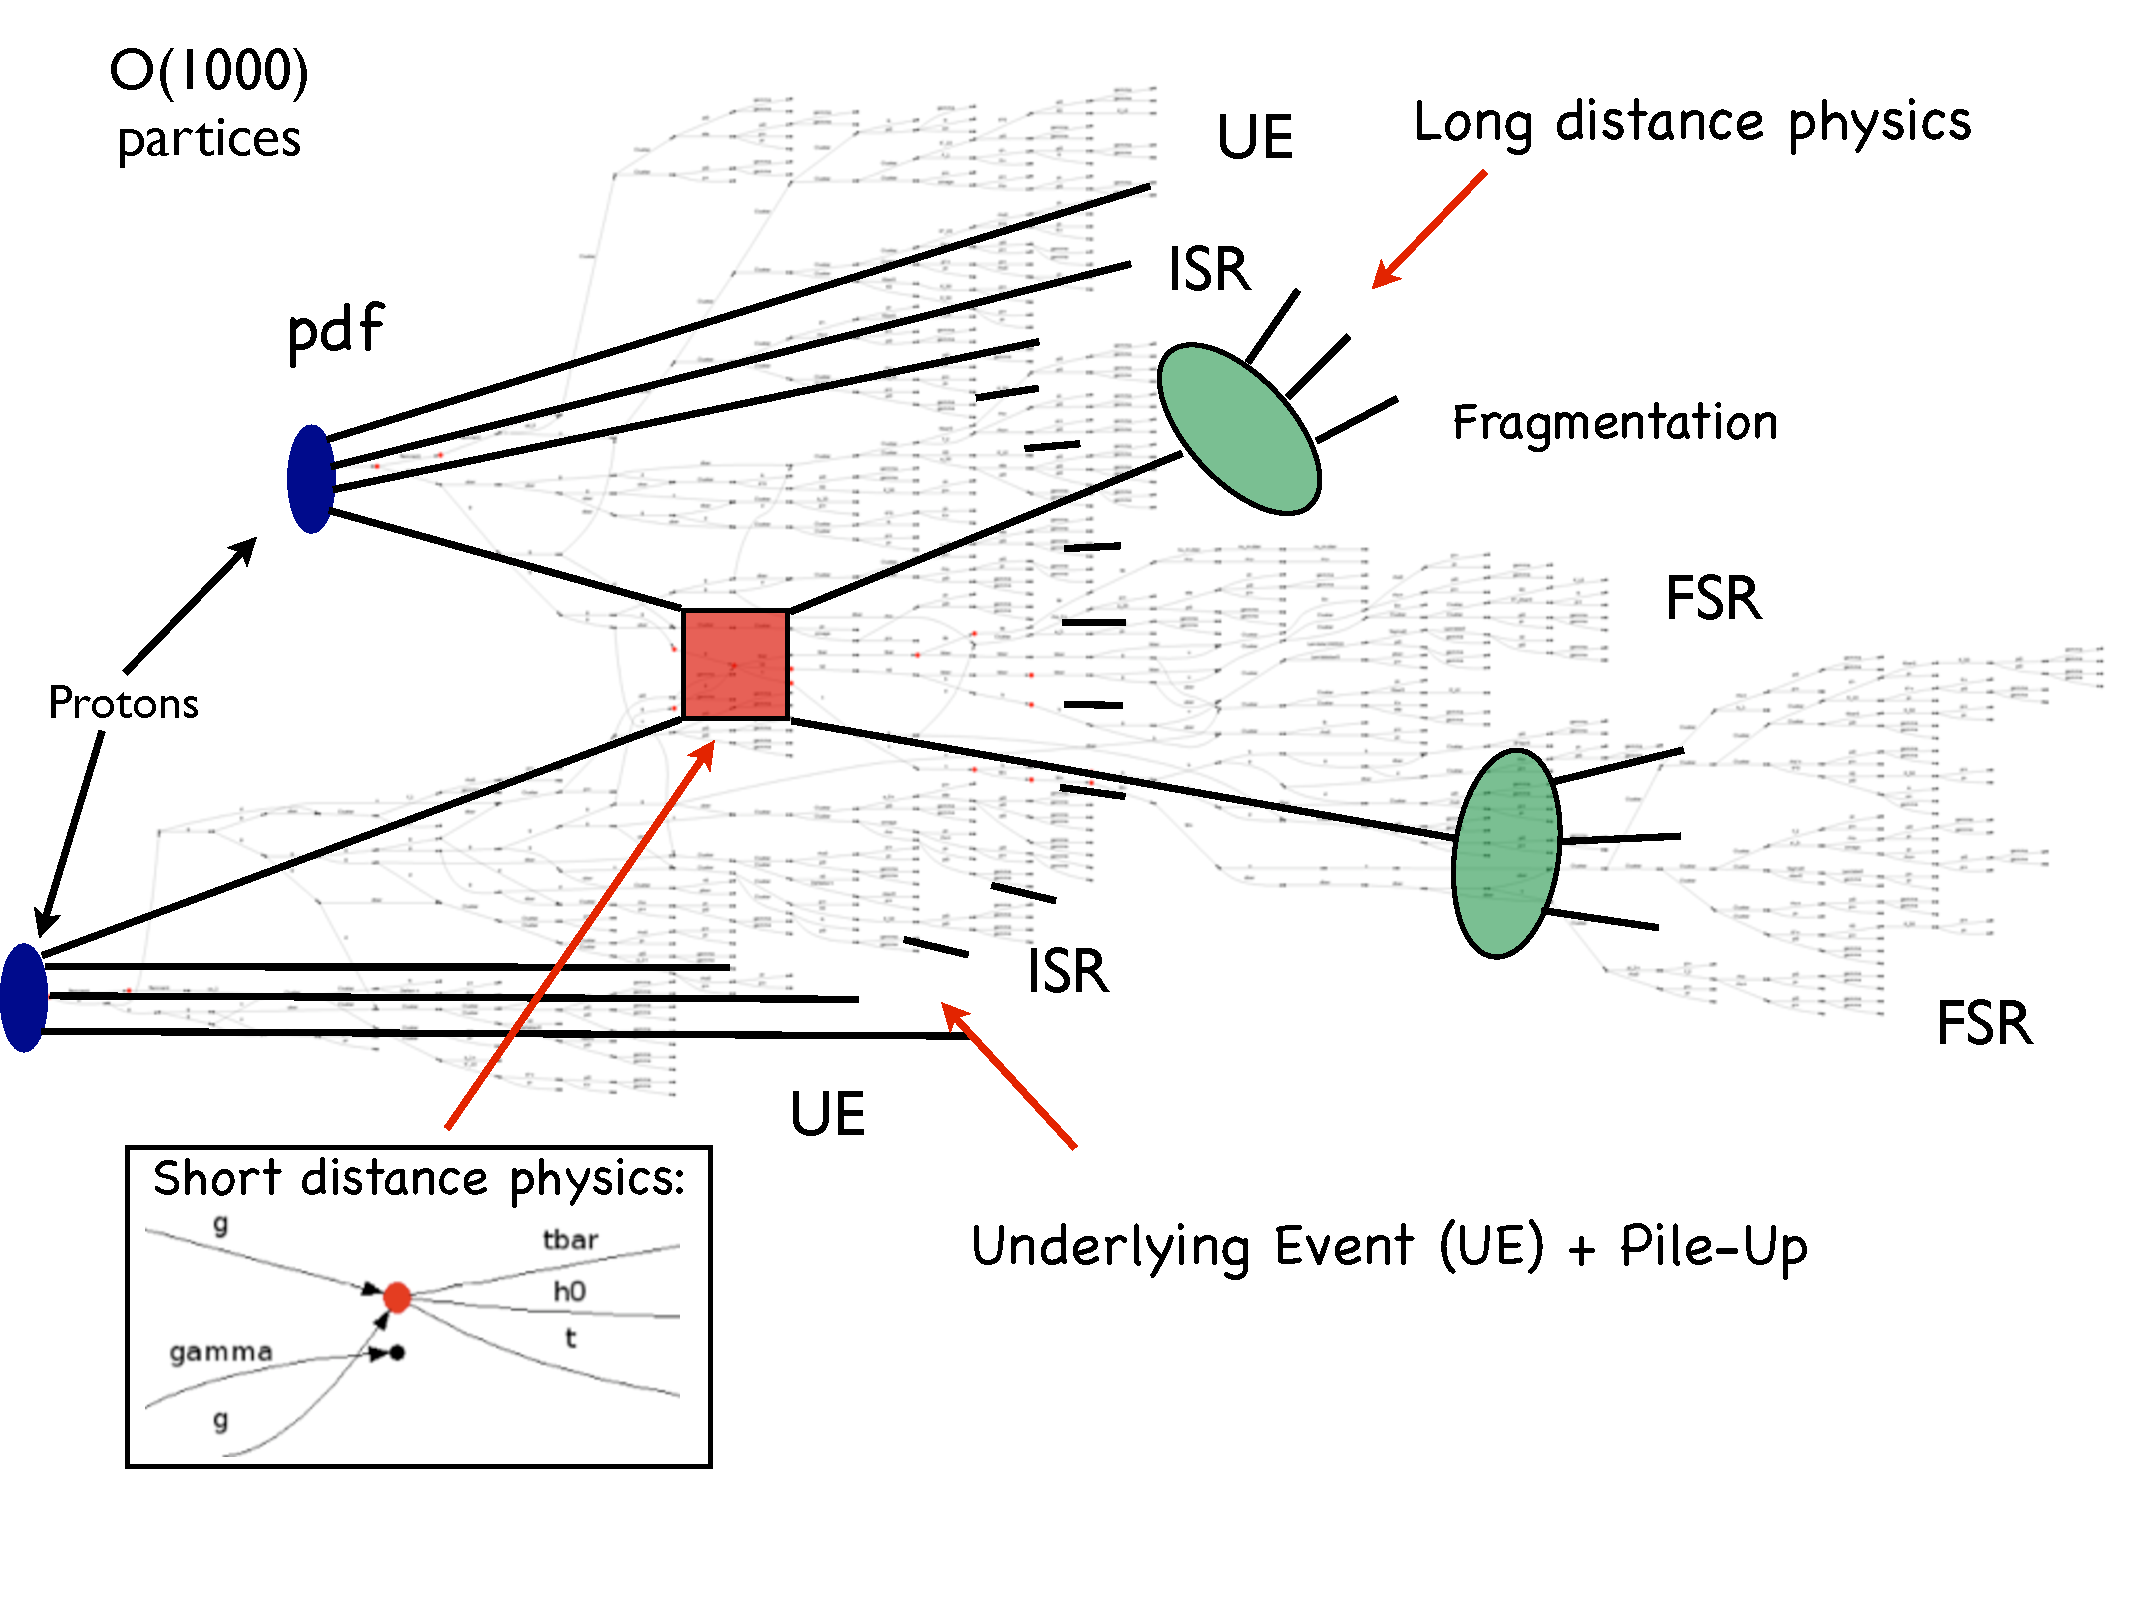
\includegraphics[scale=.4]{figures/tth}
\caption{A schematic representation of a typical high-energy proton-proton collision.}
\label{fig:tth_event}
\end{center}
\end{figure}



A remarkable feature of QCD is the fact that the strong coupling $\as= g_s^2/4 \pi$ is a decreasing function
of the energy involved in the process.
For this reason QCD has a
low energy regime, in which the theory is strongly-interacting and
a high-energy one, in which it is asymptotically free. This implies
that strong processes are computable in perturbation theory
if a sufficiently high-energy scale is involved. 
%
Thus, asymptotic freedom provides the theoretical justification of the parton model, which can be understood as the lowest
order approximation of a perturbative QCD calculation.


The theoretical description of high energy collisions of protons is fairly complex. In a typical event hundreds of particles are produced, as depicted in Fig.~\ref{fig:tth_event}.
%
The short-distance, \ie high-energy, part of the process can be computed using perturbation theory, however long-distance physics is driven by the non-perturbative nature of QCD at low energy scales. 
%
Fortunately, there exists a theorem in QCD that enables us to separate
the perturbative, \ie calculable, part of a process from the
non-perturbative one, which can be described in terms of parton
distribution (or fragmentation) functions. These objects essentially
generalise the probability distributions introduced by the parton
model.  Parton distributions are universal, \ie they do not depend on
the particular process, and they can be determined by fitting data
from previous experiments. This is the collinear factorisation theorem
and although it has been explicitly proven only for a few processes
(deep inelastic scattering of an electron off a proton and the
Drell-Yan process), it is usually considered valid and is used
ubiquitously in perturbative QCD calculations.\footnote{However,
  examples of short-distance processes that exhibits collinear
  factorisation breaking have been identified and
  studied~\cite{Forshaw:2006fk,Forshaw:2008cq,Catani:2011st,Forshaw:2012bi}.}
%
In collinear factorisation, the total cross section of inelastic proton-proton scattering to produce a final state $n$ can be calculated with the formula 
\begin{equation}
\sigma = \sum_{a,b} \int_0^1 dx_a dx_b \int d\Phi_n f_a^{h_1}(x_a,\mu_F) f_b^{h_2}(x_b, \mu_F) \frac{1}{2 \hat{s}} |\mathcal{M}_{ab \to n}|^2(\Phi_n;\mu_F,\mu_R)\;,
\label{eq:master}
\end{equation}
where $f_a^h(x,\mu)$ denotes the parton distribution functions, which depend  on the longitudinal momentum fraction $x$ of parton $a$ with respect to its parent hadron $h$, and on an arbitrary energy scale called factorisation scale $\mu_F$. In the above equation, $d\Phi_n$ denotes the differential phase space element over $n$ final-state particles,
\begin{equation}
d\Phi_n = \prod_{i=1}^{n} \frac{d^3p_i}{(2\pi)^3 2 E_i} (2 \pi)^4 \delta^{(4)}(p_a + p_b - \sum_{i=1}^{n} p_i)\;,
\label{eq:dLIPS}
\end{equation}
where $p_a$ are $p_b$ are the initial-state momenta.
The convolution of the squared matrix element $|\mathcal{M}_{ab\to
  n}|^2$, averaged over initial-state spin and colour degrees of
freedom, with the Lorentz-invariant phase space $\Phi_n$ and
multiplied by the flux factor $1/(2 \hat{s}) = 1/(2 x_a x_b s)$
results in the calculation of the parton-level cross section
$\hat{\sigma}_{ab \to n}$. The {\it cross section master formula} of
Eq.~(\ref{eq:master}) holds to all orders in perturbation theory, up
to terms which are suppressed by
$\left(\frac{\Lambda_\text{QCD}^2}{Q^2_\text{min}}\right)^p$, where $\Lambda_\text{QCD}$ is the non-perturbative QCD scale, $Q_\text{min}$ is the minimum hard energy scale
probed by the process, and typically $p=1$.  
For instance, in the case of the inclusive jet cross-section, we typically have $Q_\text{min}=p_t$, the jet transverse momentum. 
In what follows we will spend plenty of time discussing the invariant mass $m$ of a jet with
large transverse momentum $p_t$. In that case, we will be able to
identify $Q_\text{min}=m$.
%


Protons consist of many partons, each carrying a fraction of the
total proton energy. The partons of the two protons that interact with
each other via a large momentum transfer and the wide gap between this hard scale the proton mass scale is typically filled by the emission of extra partons, which is usually referred to as {\it initial state radiation}. 
Furthermore, because the hard momentum transfer can be much smaller than the proton collision energy (13 TeV), initial-state radiation is not necessarily soft.
%
In the hard process, large interaction scales and momentum transfers are probed. New heavy particles can be produced and novel interactions can be tested. Thus, the nature of the hard interaction process leaves a strong imprint in the topological structure and the composition of the whole final state.
However, if colour-charged particles\footnote{We are focusing here on QCD-induced parton showers. EW interactions can also give rise to parton showers, however, due to $\alpha \ll \alpha_s$ their contributions are suppressed. 
%
However, it should be noted the impact of EW corrections increases with the energy and so it becomes imperative to consistently include them in order to perform accurate phenomenology  at future higher-energy colliders.} are produced during the hard interaction process, they are likely to emit further partons, \ie {\it final state radiation}, to evolve from the hard interaction scale down to the hadronisation scale $\mathcal{O}(\Lambda_\mathrm{QCD})$, where non-perturbative processes rearrange the partons into colour-neutral hadrons. 

The proton's energy carried by the
spectator partons, \ie partons of the proton that are not considered
initial states of the hard interaction process, is mostly directed
into the forward direction of the detector, but a non-negligible
amount of radiation off these spectator partons can still end up in
the central region of the detector. This so-called Underlying
  Event (UE), contributing to the measured radiation in a detector,
is, on average, softer, \ie has lower transverse momentum, than for
example the decay products of the hard process or initial state
radiation. For jet substructure observables, however, it plays an
important role as it can complicate the extraction of information from
observables that rely on the details of the energy distribution inside
a jet.


Furthermore, protons are accelerated and collided in bunches.
%
When two bunches of protons cross at an interaction point, multiple
proton-proton collisions can occur simultaneously. What is observed in
the detectors is therefore a superposition of these many events.
%
When one of these collisions is hard and deemed interesting enough by
the experiments' triggers to be stored on tape, it therefore
overlays in the detector with all the other simultaneous, mostly
soft, collisions.
%
This effect is known as pileup and presents a challenge to the
reconstruction of the objects seen in the detectors in general and of
the hadronic part of the event, in particular.
%
To give a quantitative estimate, at the end of Run II of the LHC (late
2018), the machine delivers a luminosity
${\cal L}\sim 2\times 10^{34}\:\text{cm}^{-2}\text{s}^{-1}$ which, for a
bunch spacing of $25$ nanoseconds and a typical total proton-proton
cross-section of $100$~mb, corresponds to an average of 50 interactions
per bunch-crossing (assuming that they are Poisson-distributed).
%
We refer the interested reader to a recent review on this subject in
the context of jet physics, written by one of us~\cite{Soyez:2018opl}.

\section{Generalities on perturbative calculations}\label{sec:generalities}


The calculation of the matrix element in Eq.~(\ref{eq:master}) is
usually approximated by a perturbative series in powers of the strong
coupling, henceforth the \emph{fixed-order} expansion. The evaluation
of such perturbative expansion, and more generally the development of improved
techniques to compute {\em amplitudes}, is one of the core activities of QCD phenomenology. 
%
In this framework, theoretical precision is achieved by computing cross-sections $\sigma$ including increasingly higher-order corrections in the strong coupling $\as$
\begin{equation} \label{fixedorder_sigma}
\sigma\left(v\right) = \sigma_0 + \as \, \sigma_1 +\as^2 \, \sigma_2 +\as^3 \, \sigma_3 + \ord(\as^4),
\end{equation}
where $v$ is a generic observable, which for definiteness we take dimensionless. In the above expression leading order (LO) contribution $\sigma_0$ is the Born-level cross section for the scattering process of interest. Subsequent contributions in the perturbative expansion $\sigma_i$ constitute the next-to$^i$-leading (N$^i$LO) corrections. In the language of Feynman diagrams, each power of $\as$ corresponds to the emission of a QCD parton, either a quark or a gluon, in the final state or to a virtual correction. 
%
The theoretical community has put a huge effort in computing higher-order corrections. LO cross-sections can be computed for an essentially arbitrary number of external particles. Automation has been achieved in recent years also for NLO calculations and an increasing number of NNLO calculations is now available in computer programs. 
%
Moreover, for hadron-collider processes with simple topologies, recent
milestone calculations have achieved N$^3$LO
accuracy~\cite{Anastasiou:2015ema,Dreyer:2016oyx}. A particularly
important example which  falls under this category is the main
production channel of the Higgs boson (through gluon-gluon fusion).
%
One of the main challenges in this enterprise is the treatment of the infra-red region. As it is going to be discussed in the following, the emissions of soft and/or collinear partons is also problematic because it can generate large logarithmic terms in the perturbative coefficients, thus invalidating the fixed-order approach.

%
It is well known that the calculations of Feynman diagrams is plagued by the appearance of divergences of different nature. 
%
Loop-diagrams can exhibit ultra-violet singularities. Because QCD is a renormalisable theory, such infinities can be absorbed into a redefinition of the parameters that enter the Lagrangian, \eg the strong coupling $\as$.
%
Moreover, real-emission diagrams exhibit singularities in particular
corners of the phase-space. More specifically, the singular
contributions have to do with collinear, \ie small angle, splittings
of massless partons and emissions of soft gluons, off both massless and
massive particles. Virtual diagrams also exhibit analogous infra-red
and collinear (IRC) singularities and rather general
theorems~\cite{Blochnordsieck,Kinoshita,Lee} state that such
infinities cancel at each order of the perturbative series Eq.~(\ref{fixedorder_sigma}), when real and virtual corrections are added together, thus leading to observable transition probabilities that are free of IRC singularities.
%
We will explicitly discuss infra-red singularities in a NLO calculation in the next section.
%
Moreover, in order to be able to use the perturbative expansion of
Eq.~(\ref{fixedorder_sigma}), one has to consider observables
$v$ that are infra-red and collinear (IRC) safe, \ie measurable quantities that do not spoil the above theorems. We will come back to a more precise definition of IRC safety in Sec.~\ref{sec:IRC-safety}.

It is worth pointing out that, in
  practice, non-perturbative effects like hadronisation regulate
  soft and collinear divergences, so that cross-sections are
  finite. The requirement of IRC safety means that an observable can
  be computed reliably in perturbative QCD, up to non-perturbative
  power corrections, which decrease as the hard scale of the process increases.
  %
  Moreover, from an
  experimental viewpoint, the finite resolution of the detectors also acts
as a regulator, thus preventing the occurrence of actual
singularities. However, this in turn would be reflected on a possibly
strong dependence of theoretical predictions on the detector
resolution parameters, which one wishes to avoid.


The fixed-order expansion of Eq.~(\ref{fixedorder_sigma}) works well
if the measured value of the observable is $v\simeq 1$, a situation in which there is no significant hierarchy of scales.
%
However, it loses its predictive power if the measurement of
$v\ll 1$ confines the real radiation into a small corner of
phase-space, while clearly leaving virtual corrections
UE-restricted. 
%
For IRC safe observables the singular terms still
cancel, but logarithmic corrections in $v$ are
left behind, causing the coefficients $\sigma_i$ to become large, so
that $\as^i \sigma_i \sim 1$. 
Because these logarithmic corrections
are related to soft and/or collinear emissions, one can expect at most
two powers of $L=\log\big(\frac{1}{v}\big)$~\footnote{Throughout this book we denote with $\log(x)$ the natural logarithm of $x$.} for each power of the
strong coupling.
%
For example, when $v$ is sensitive
only to angles up to $\theta_\text{cut}\ll 1$, one should expect large
(collinear) logarithms of $1/\theta_\text{cut}$, and when
$v$ is sensitive only to $|k_{3\perp}|$ up to
$|k_{3\perp}^\text{cut}|\ll 1$, one should expect large (soft) logarithms of $Q/|k_{3\perp}^\text{cut}|$. 


Let us consider the {\it cumulative} cross-section for measuring a
value of the observable of interest which is less than a given value
$v$, normalised to the inclusive Born-level cross-section
$\sigma_0$.\footnote{Note that in the literature, $\Sigma$
  sometimes refers to the un-normalised cumulative cross-section.}
% i.e.\ the so-called cumulative, then
We have
\begin{align} 
  \Sigma\left(v\right)
  & = \int_0^v dv' \frac{1}{\sigma_0}\frac{d\sigma}{dv'} \\
  & = 1 + \as \, \left( \sigma_{12} L^2+\sigma_{11} L+ \dots \right)  
+\as^2 \,\left( \sigma_{24} L^4+\sigma_{23} L^3+ \dots \right)   + \ord(\as^n L^{2n}).\label{expanded_sigma}
\end{align}
All-order resummation is then a re-organisation of the above perturbative series. For many observables of interest, the resummed expression exponentiates, leading to
\begin{equation} \label{resummed_sigma}
\sigma\left(v \right) = \sigma_0 \, g_0 \exp \left[ L g_1(\as L)+g_2(\as L)+\as g_3(\as L)+ \dots \right],
\end{equation}
where $g_0$ is a constant contribution which admits an expansion in $\as$. In analogy to the fixed-order terminology, the inclusion of the contribution $g_{i+1}$, $i\ge0$, leads to next-to$^i$-leading logarithmic (N$^i$LL) accuracy.

Fixed-order Eq.~(\ref{fixedorder_sigma}) and resummed Eq.~(\ref{resummed_sigma}) expansions are complementary.
On the one hand, fixed-order calculations fail in particular limits of
phase-space, indicating the need for an all-order approach. On the
other hand, all-order calculations are only possible if particular
assumptions on the emission kinematics are made. Thus, the most
accurate theoretical description for the observable $v$ is
achieved by matching the two approaches \eg using (other so-called
{\em matching schemes} exist)
\begin{equation}\label{eq:matching-add}
\sigma^\text{matched}(v)=\sigma^\text{fixed-order}(v)+\sigma^\text{resummed}(v)-\sigma^\text{double counting}(v).
\end{equation}









\section{Factorisation in the soft and collinear limits}\label{sec:qcd_soft_fact}
\begin{figure}
\begin{center}
  \subfloat[]{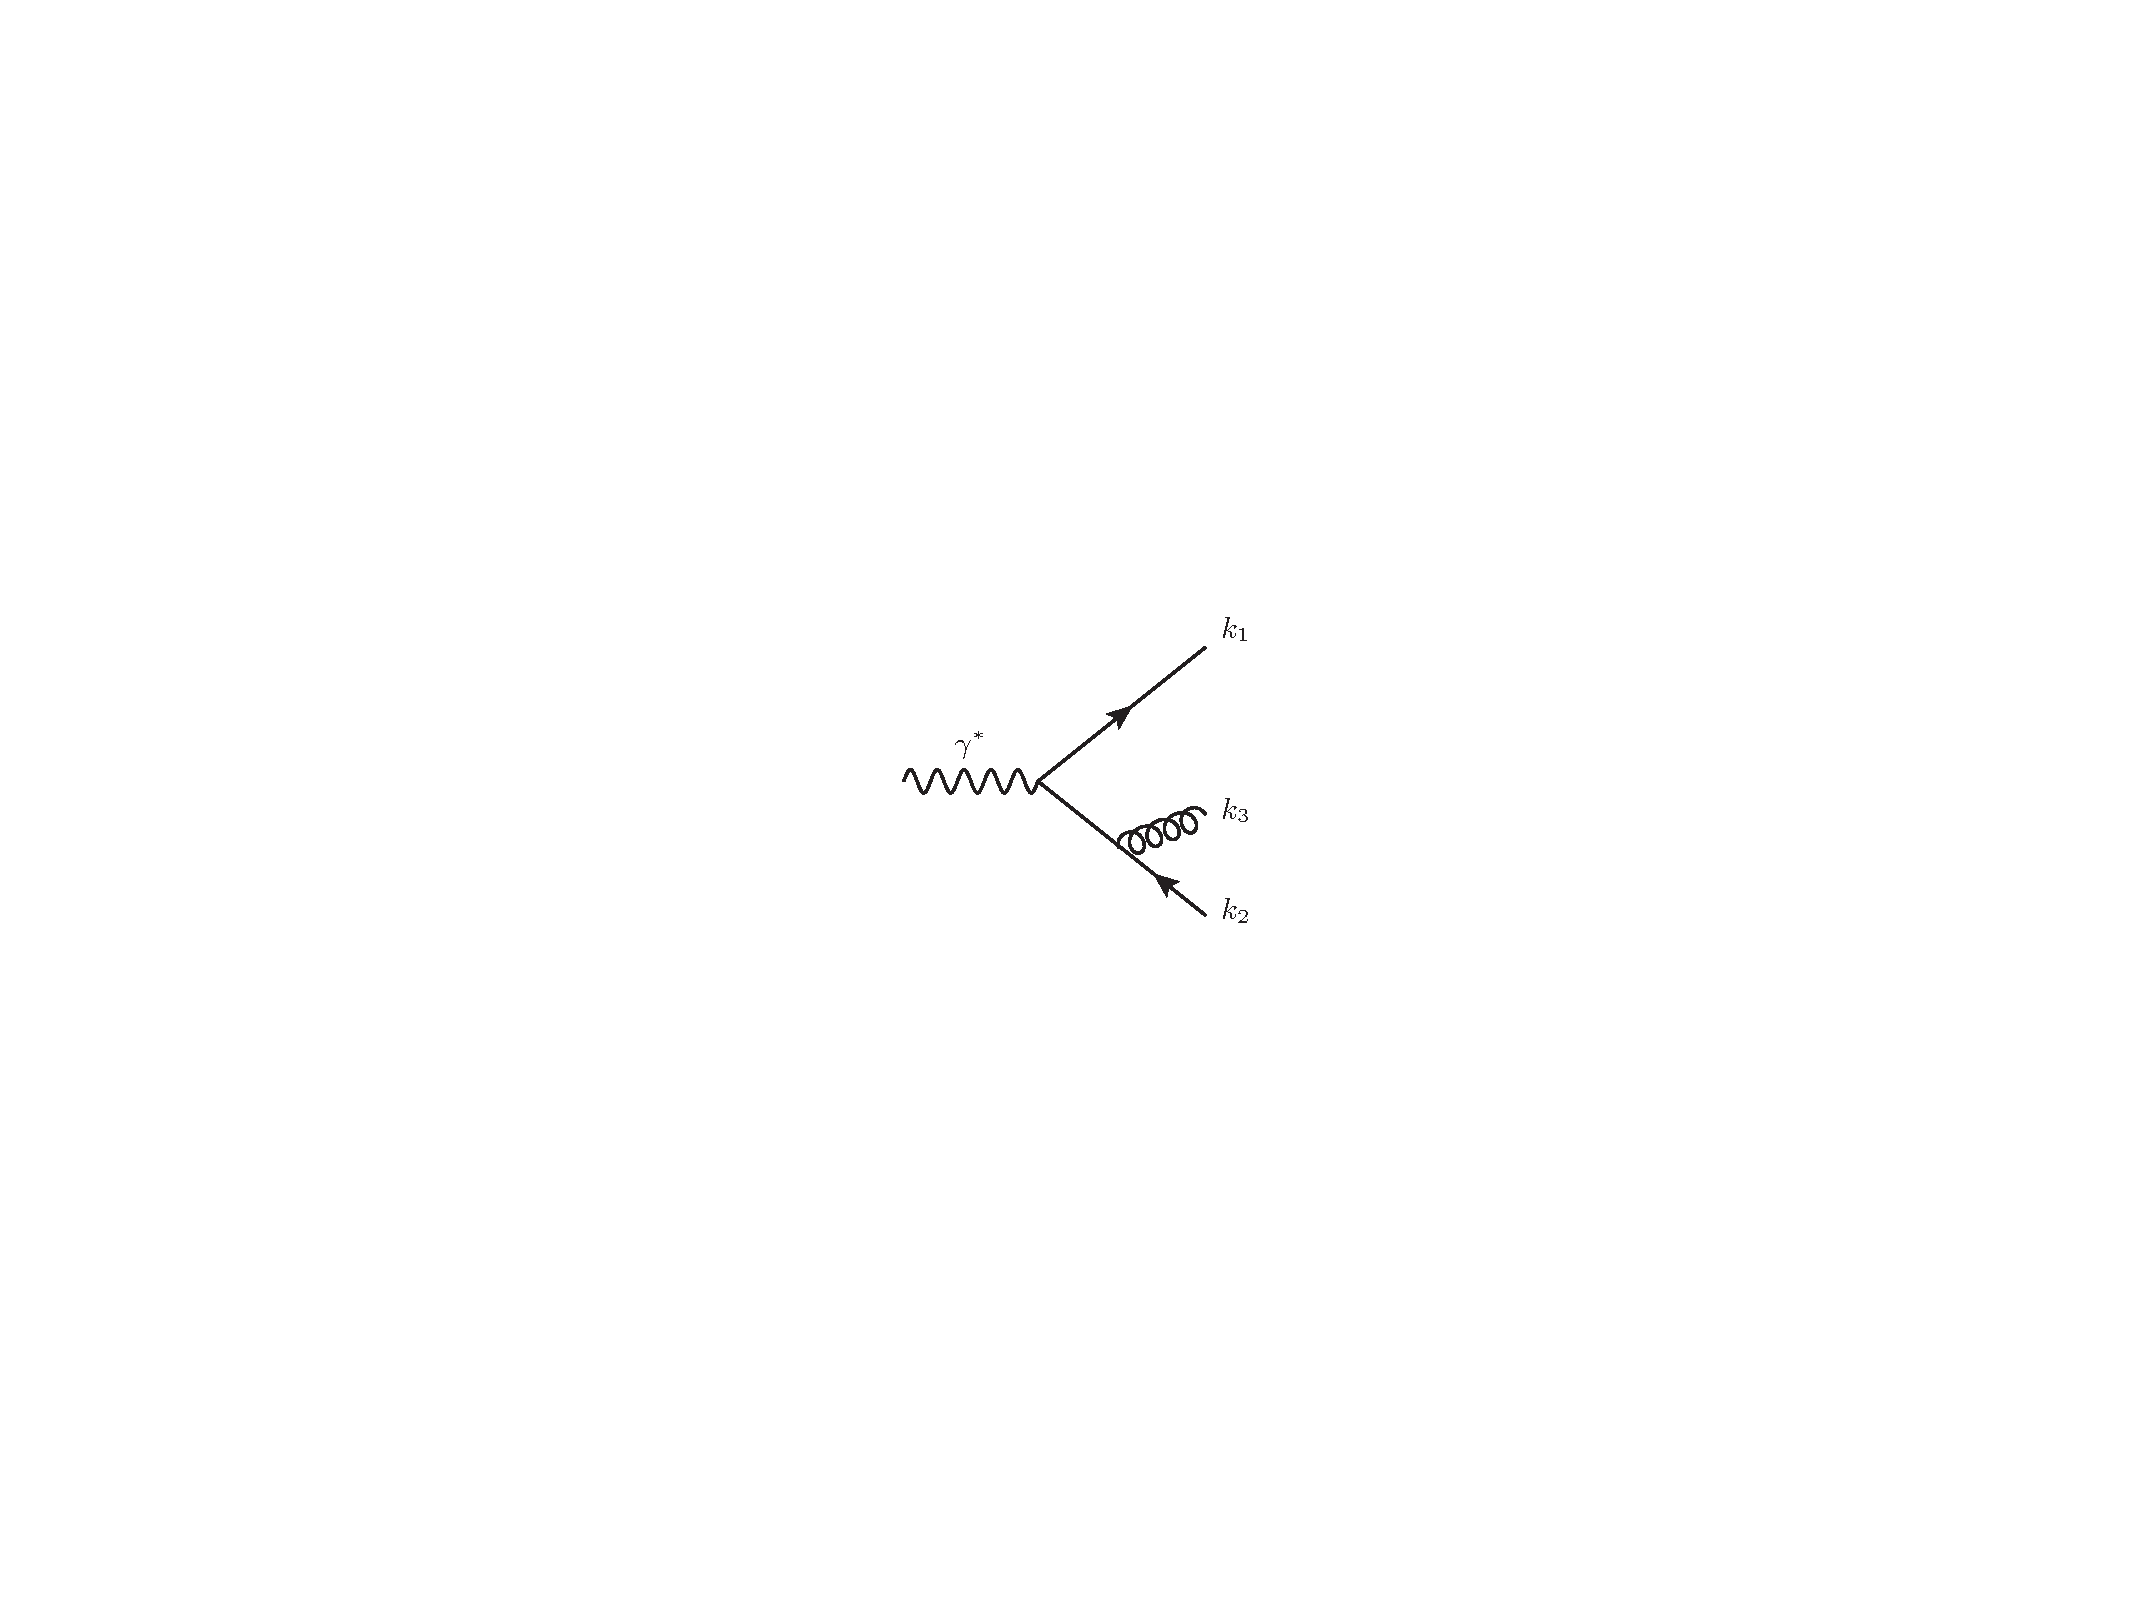
\includegraphics[scale=0.6,page=1]{figures/eenlo} \label{eenloR1}} \hfill
  \subfloat[]{\includegraphics[scale=0.6,page=2]{figures/eenlo} \label{eenloR2}} \hfill
  \subfloat[]{\includegraphics[scale=0.6,page=3]{figures/eenlo} \label{eenloV}} 
\caption{Feynman diagrams contributing to the cross-section of
  $e^{+}e^{-}\to q\bar{q}$ at $\mathcal{O}(\alpha_s)$.}\label{fig:sigma_nlo}
\end{center}
\end{figure}

In order to highlight the structure of IRC singularities in matrix elements, we consider the calculation of the NLO QCD corrections in the soft limit. For this presentation we closely follow the review~\cite{Luisoni:2015xha}.
%
In order to simplify our discussion, rather than presenting a
calculation for proton-proton collisions, for which we would have to
include parton distribution functions and  discuss how to treat
initial-state radiation, we focus our discussion on a process in
electron-positron collisions, for which we can concentrate on QCD
radiation off the final-state quarks. We will show that the requirement of
  IRC safety implies with some constraints on observables to guarantee
  the cancellation of divergences when combining real and virtual
  diagrams. Furthermore, we will also see that, if we consider an
inclusive observable, we obtain an NLO correction which is free of
large logarithms.

Let us therefore consider the $\mathcal{O}(\as)$ correction to the process
\begin{equation}
e^+ e^- \to \gamma^* \to  q \bar q.
\end{equation}
The relevant Feynman diagrams are shown in Fig.~\ref{fig:sigma_nlo}, where for convenience we have dropped the initial-state lepton line. 
% 
We label the momentum of the quark and anti-quark $k_1$ and $k_2$,
respectively, and we start by considering the real emission of a soft
gluon with momentum $k_3$, \ie diagrams in Fig.~$\ref{eenloR1}$ and Fig.~$\ref{eenloR2}$.
%
The matrix element for diagram $(b)$ can be written as
\begin{eqnarray}
M_{3}^{(b)}&=&t_{1}^{a}\,\gstrong\, \bar{u}\left(k_1\right)\gamma^{\mu}\e^*_{\mu}\left(k_3\right)\frac{\slashed{k}_1+\slashed{k}_{3}}{\left(k_1+k_3\right)^{2}+i\epsilon}\tilde{M}_{2}\nonumber\\
&\stackrel{k_3\to 0}{\longrightarrow}&t_{1}^{a}\,\gstrong\, \bar{u}\left(k_1\right)\gamma^{\mu}\e^*_{\mu}\left(k_3\right)\frac{\slashed{k}_{1}}{2 k_1 \cdot k_3+i\epsilon}\tilde{M_{2}}\nonumber\\%\angIn{M_{k_3\bar{k_3}}'}\nonumber\\
&=&t_{1}^{a}\,\gstrong\, \frac{k_1^{\mu}}{k_1\cdot k_3}\e^*_{\mu}\left(k_3\right)  \bar{u}\left(k_1\right) \tilde{M_{2}}
=t_{1}^{a}\,\gstrong\, \frac{k_1^{\mu}}{k_1\cdot k_3}\e^*_{\mu}\left(k_3\right)  {M_{2}},
\end{eqnarray}
where we have used anti-commutation relations of the Dirac matrices and $\slashed{k_1}u(k_1)=0$ to get the last line.
%
The factor $k_1^{\mu}/(k_1\cdot k_3)$ is called eikonal factor and $t_{1}^{a}$ is the colour charge associated to the emission of a gluon off a quark line, \ie it is a generator of SU(3) in the fundamental representation. We have also used fairly standard notation for the Dirac spinor $\bar u(k)$ and for the gluon polarisation vector $\e_\mu(k_3)$. In the last step the Dirac spinor was absorbed in the 2-parton matrix element $M_2$ and therefore we dropped the tilde on it. For the full real-emission amplitude we find
%
\begin{equation}\label{eq:softfactorisation}
M_{3}=M_{3}^{(a)}+M_{3}^{(b)}\stackrel{k_3\to 0}{\longrightarrow} g_s  J^{\mu}\left(k_3\right)\e^*_{\mu}\left(k_3\right)M_{2},
\end{equation}
where we have introduced the eikonal current
\begin{equation}\label{eq:eikonalcurrent}
J^{\mu}\left(k\right)=\sum_{i=1}^{2}t_i^{a}\frac{k_i^{\mu}}{k\cdot k_i}.
\end{equation}
It is important to note that the factorisation does not depend on the internal structure of the amplitude. From the physical point of view, this reflects the fact that the large wavelength of the soft radiation cannot resolve the details of the short distance interactions. However, the proof of this statement to any perturbative orders is highly non-trivial and it heavily relies on gauge invariance.


We now square the amplitude and we arrive at the following factorised
expression for the emission of a soft real gluon
\begin{eqnarray}\label{eq:eikonalfactorisation}
\left|M_3\right|^{2}&\stackrel{k_3\to 0}{\longrightarrow} &\left|M_2\right|^{2}g_s^{2} J^{\mu}\left(k_3\right)J^{\nu}\left(k_3\right)\left(-g_{\mu\nu}\right)\nonumber\\
&=&\left|M_2\right|^{2}g_s^{2} \left[-\sum_{i,j}t_{i}^{a}t_{j}^{a}\frac{k_i\cdot k_j}{(k_i\cdot k_3)(k_j\cdot k_3)}\right]\nonumber\\
&=&\left|M_2\right|^{2}g_s^{2}  C_{12}\frac{k_1\cdot k_2}{(k_1\cdot k_3)(k_2\cdot k_3)},
\end{eqnarray}
where we have introduced the effective colour charge
\begin{equation}\label{eq:eff-col-def}
C_{ij}= - 2 \, t_{i}^{a}\, t_{j}^{a}.
\end{equation}
We note that the effective colour charge is a matrix which has in principle non-zero entries also away from the diagonal. It is easy to show using colour conservation that its structure noticeably simplifies in the case under consideration, because we only have two hard legs which carry colour:
\begin{equation}
t^a_1+t^a_2=0 \Longrightarrow \left({t_1^a}\right)^2+\left({t_2^a}\right)^2= - 2 t_1^a t_2^a  \Longrightarrow C_{12}= 2\cf,
\end{equation}
where all the above equalities are meant to hold when the matrices act on physical states.
The effective colour charge turns out to be diagonal also in the case of three hard coloured legs, as we shall see in Sec.~\ref{sec:Zjet}, while with four or more hard partons a non-trivial matrix structure emerges.
We point out for the interest reader that a general and rather powerful colour-operator formalism to deal with this issue exists~\cite{Catani:1985xt,Catani:1996vz,Catani:1996jh,Dokshitzer:2005ig,Dokshitzer:2005ek}.

The soft approximation can be applied also to the virtual
corrections. i.e.\ to the diagram in Fig.~\ref{eenloV}. In this limit we can in general neglect powers of the
loop momentum $k_3$ in the numerator.  Moreover, in the denominator we can use the fact that $k_3^{2}\ll k_i\cdot k_3$. The loop correction to quark-antiquark pair production is therefore proportional to
\begin{eqnarray}
I&=&g_s^{2} \cf(-i)\int\frac{d^{4}k_3}{(2\pi)^{4}}\frac{\bar{u}\left(k_1\right)\gamma^{\mu}\left(\slashed{k}_1+\slashed{k}_3\right)\gamma^{\rho}\left(\slashed{k}_3-\slashed{k}_2\right)\gamma_{\mu}v\left(k_2\right)}{\left[\left(k_3+k_1\right)^{2}+i\epsilon\right]\left[\left(k_3-k_2\right)^{2}+i\epsilon\right]\left[k_3^{2}+i\epsilon\right]}\nonumber\\
&\to&g_s^{2} \cf(-i)\int\frac{d^{4}k_3}{(2\pi)^{4}}\frac{\left(k_1\cdot k_2\right)\left[\bar{u}\left(k_1\right)\gamma^{\rho}v\left(k_2\right)\right]} {\left[k_3\cdot k_1+i\epsilon\right]\left[-k_3\cdot k_2+i\epsilon\right]\left[k_3^{2}+i\epsilon\right]},
\end{eqnarray}
where we have written the result in $d=4$ space-time dimensions
because we are going to combine it together with the real-emission
part, before calculating the divergent integrals.

It is helpful to use the following parametrisation of the four-momenta:
\begin{equation}
k_1^{\mu}=E_1\left(1,0,0,1\right)\,,\quad k_2^{\mu}=E_2\left(1,0,0,-1\right)\,,\quad k_3^{\mu}=\left(k_{3}^0,\vec{k}_3\right)\,\textrm{ with }\, \vec{k}_3=\left(\vec{k}_{3\perp},k_{3}^z\right)\,,
\end{equation}
where $\vec{k}_{3 \perp}$ is the vectorial transverse loop momentum and $k_{3\perp} \equiv | \vec{k}_{3\perp} |$.
%
We note that
\begin{equation}\label{eq:dipole-kperp}
  k_{3\perp}^2=\frac{2(k_1.k_3)(k_3.k_2)}{(k_1.k_2)}.
\end{equation}
% 
We thus obtain
\begin{equation}\label{eq:loopintsoft}
I=g_s^{2} \cf(-i)\int\frac{d^{3}k_3}{(2\pi)^{4}}\frac{2\:d k_3^0 \left[\bar{u}\left(k_1\right)\gamma^{\rho}v\left(k_2\right)\right]}{\left(k_3^0-k_3^z+i\epsilon\right)\left(-k_3^0-k_3^z+i\epsilon\right)\left({k_3^0}^{2}-{k_3^z}^{2}-k_{3 \perp}^{2}+i\epsilon\right)}
\end{equation}
When performing loop-calculations, one usually introduces a regulator,
such as for instance dimensional regularisation, and then evaluates
the integrals in Eq.~(\ref{eq:loopintsoft}) directly. Here we take
another approach which allows us to highlight the similarities between loop integrals for the
  virtual terms and phase-space integrals for the real
  contributions. We want first to evaluate the integral in
$k_3^0$. We note that the integrand has four poles in the complex
$k_3^0$ plane, which are located at 
\begin{eqnarray}
k_3^0=k_3^z-i\epsilon,\qquad k_3^0=-k_3^z+i\epsilon, \qquad k_3^0=\pm\left(|\vec{k_3\,}|-i\epsilon\right)\,.
\end{eqnarray}
Closing the contour from below we find
\begin{equation}\label{eq:virtual-antenna+glauber}
I=g_s^{2} \cf\left[\bar{u}\left(k_1\right)\gamma^{\rho}v\left(k_2\right)\right]\int\frac{d^{3}k_3}{(2\pi)^{3}}\left[\frac{-\left(k_1\cdot k_2\right)}{2|\vec{k_3\,}|\left(k_1\cdot k_3\right)\left(k_2\cdot k_3\right)}-\frac{1}{\left(k_3^z-i\epsilon\right)\left(k_{3\perp}^{2}\right)}\right]\,,
\end{equation}
where the second integral is a pure phase
\begin{equation}
\int\frac{d k_3^z\, d^2 k_{3\perp}}{\left(2\pi\right)^{3}}\frac{1}{\left(k_3^z-i\epsilon\right)\left(k_{3\perp}^2 \right)}=-\int d k_3^z\frac{k_3^z+i\epsilon}{{k_3^z}^{2}+\epsilon^{2}}\int\frac{d k_{3\perp}}{\left(2\pi\right)^{2}}\frac{1}{k_{3\perp}}=-\int\frac{\left(i\pi\right)}{\left(2\pi\right)^{2}}\frac{d k_{3\perp}}{k_{3\perp}}\,.
\end{equation}
This contribution is usually referred to as the Coulomb, or Glauber,
phase. We note that the above phase always cancels when considering
physical cross-sections in Abelian theories like QED. However, it can
have a measurable effect in QCD cross-sections, in the presence of a
high enough number of harder coloured legs, which lead to a
non-trivial matrix structure for the effective colour charges
Eq.~(\ref{eq:eff-col-def}).


Collecting real and virtual contributions together, we can compute the
NLO distribution of an observable $v$ by introducing an
appropriate measurement function
$V_{n}\left(\left\{k_i\right\}\right)$, which describes
%
the value of the observable for a set of $n$ final-state particles
$k_1,\dots,k_n$.
%
The measurement function can contain Dirac delta corresponding to
constraints imposed in differential distributions, and/or Heaviside
$\Theta$ functions, for example when one imposes cuts on the
final-state or if one works with cumulative distributions.
%
Furthermore, if we are dealing with jet observables, the measurement
functions must also tell us how to combine particles in a jet, \ie it
must specify the jet algorithm
(cf.~Chapter~\ref{chap:jets-and-algs}).\footnote{Technically, the jet
  clustering can usually be written as a series of $\Theta$
  functions.}  With this in mind, we can write the cross-section for
an observable $v$ to NLO accuracy as the sum of three contribution:
Born, real emission and virtual corrections:
\begin{align}\label{eq:real-virtual-together}
\sigma\left(v\right)&=\frac{1}{2s}\int d\Phi_2\left|M_2\right|^{2}V_2\left(k_1,k_2\right)\\
&+\frac{1}{2s}\int d\Phi_2\left|M_2\right|^{2}\int\frac{d^{3}k_3}{(2\pi)^{3}2 | \vec{k}_3|}2 g_s^{2}\cf\frac{\left(k_1\cdot k_2\right)}{\left(k_1\cdot k_3\right)\left(k_2\cdot k_3\right)}
  \left[V_{3}\left(k_1,k_2,k_3\right)-V_2\left(k_1,k_2\right)\right].\nonumber
\end{align}
We note that the Born contribution and the one-loop corrections live in the two-particle phase-space and are characterised by the same measurement function. Instead, the real emission contribution live in a three-body phase-space and, consequently, the measurement function is the three-particle one. 


The main result of our discussion so far is Eq.~(\ref{eq:real-virtual-together}), which describes the behaviour of a typical NLO cross-section in the limit where the radiated parton (gluon) is soft. However, if we take a closer look we note that 
\begin{equation}
k_i \cdot k_3 = E_i E_3 (1-\cos \theta_{i3}), \quad i=1,2.
\end{equation}
Thus, the eikonal factor exhibits a singularity not only in the soft limit but also when the parton with momentum $k_3$ becomes collinear with either $k_1$ or $k_2$.
It is clear that, while the eikonal approximation is sufficient to
correctly capture both the soft-collinear and soft wide-angle, we have to extend our formalism in order to include also the relevant hard-collinear terms. It must be noted that the collinear limit is in many respects easier than the soft limit discussed so far, essentially because the collinear factorisation emerges from a semi-classical picture whereby a parent parton splits into two daughters. An important consequence of this fact is that collinear singularities are always accompanied by diagonal colour charge $C_{ii}$, which is the Casimir of the relevant splitting, \ie  $C_F$ for quark splittings and $C_A$ for gluon splittings.\footnote{We warn the reader that although physically motivated, this statement is all but trivial to show!
 After the first splitting the total colour charge will be shared among the two partons and further radiation can be emitted from either of them.
 This leads to a colour radiation pattern which is in principle rather complicated.
 However, soft radiation cannot resolve the details of the interaction
 which happens at shorter distance and higher momentum scale, a
 phenomenon called \emph{coherence}. Therefore a soft gluon emitted at
 an angle $\theta$ will only see the total colour charge of the
 radiation emitted at smaller angles~\cite{Ermolaev:1981cm,Mueller:1981ex,Bassetto:1982ma}. 
 The iteration of this argument essentially leads angular-ordered
 parton showers and to the resummation of large logarithms in the
 framework of the coherent branching
 algorithm~\cite{Catani:1990rr,Catani:1992ua}.} 
 The splitting of a quark into a gluon with momentum fraction $z$ and
 a quark with momentum fraction $1-z$ $q \to q g$ is described at LO by the
 splitting function
 \begin{equation}\label{eq:quarksplitting}
 P_q(z)=C_F\frac{1+(1-z)^2}{z},
 \end{equation}
 while the gluon splitting into a pair of gluons or a quark-antiquark pair reads
 \begin{equation}\label{eq:gluonsplitting}
% P_g (z)=C_A \left[ \frac{1-z}{z}+\frac{z(1-z)}{2}+\frac{n_f T_R}{2C_A}\left(z^2+(1-z)^2\right),
  P_g (z)=C_A \left[ 2\frac{1-z}{z}+z(1-z)+\frac{n_f T_R}{C_A}\left(z^2+(1-z)^2\right)
 \right].
 \end{equation}
 where the first contribution describes the splitting $g \to gg$,
 while the second one, proportional to $n_fT_R$ with $n_f$ the number
 of massless flavours, corresponds to the splitting $g \to q \bar q$.
 We note that both Eqs.~(\ref{eq:quarksplitting})
 and~(\ref{eq:gluonsplitting}) exhibit a $z \to 0$ singularity which
 is the soft singularity of Eq.~(\ref{eq:real-virtual-together}),
 while the finite-$z$ part of the splitting functions describe the
 hard-collinear contribution.

 \section{Infra-red and collinear safety}\label{sec:IRC-safety}


We are now ready to discuss infra-red and collinear safety in a more detailed way. Let us go back to Eq.~(\ref{eq:real-virtual-together}), or alternatively we could consider its extension in the collinear limit.  In order to achieve a complete cancellation of the IRC singularities, we must consider observables $V$ that satisfy the following properties, which we take as the definition of IRC safety~\cite{Sterman:1977wj}:
\begin{align}
\text{collinear safety:}&&
V_{m+1}\left(\ldots,k_i,k_j,\ldots\right)&\longrightarrow V_{m}\left(\ldots,k_i+k_j,\ldots\right) &&\mathrm{if}\;k_i\parallel k_j ,\\
\text{infrared safety:}&&
V_{m+1}\left(\ldots,k_i,\ldots\right)&\longrightarrow V_{m}\left(\ldots,k_{i-1},k_{i+1},\ldots\right) &&\mathrm{if}\;k_i\to 0.
\end{align}
In words, whenever a parton is split into two collinear partons, or
whenever an infinitesimally soft parton is added --- \ie in situations
where an extra emission makes the real amplitude divergent --- the value
of the observable must remain unchanged, in order to guarantee a
proper cancellation of the divergence against virtual corrections.
%
The above limits have to hold not only for a single particle, but for an ensemble of partons becoming soft and/or collinear.
IRC safe properties of jet cross-sections and related variables, such as event shapes and energy correlation functions were first studied in Refs.~\cite{Sterman:1978bi,Sterman:1978bj,Sterman:1979uw}.
%


Let us consider first the case of inclusive observables, \ie observables
that do not constrain additional radiation. We then have
$V_m\left(k_1,\ldots,k_m\right)=1$ for all $m$ and the cancellation is
complete. Consequently, the total cross-section remains unchanged by
the emission of soft particles, as it should. 
Note that
  Eq.~(\ref{eq:real-virtual-together}) is computed in the soft
  limit. An exact calculation involves additional corrections,
  non-divergent in the soft limit, so that the NLO contribution is a
  finite ${\cal{O}}(\alpha_s)$ correction.
%
Finally, and more interestingly for the topic of this book, let us consider the case of an exclusive (but IRC safe) measurement. Although the singularities cancel, the kinematic dependence of the observable can cause an imbalance between real and virtual contributions, which manifests itself with the appearance of potentially large logarithmic corrections to any orders in perturbation theory.
%
As we have previously mentioned, these logarithmic become large if
$v\ll 1$, \ie if the measurement function constrains real
radiation in a small corner of phase-space.
%
These contributions spoil
the perturbative expansion in the strong coupling and must be resummed
to all orders in order to obtain reliable theoretical predictions for
exclusive measurements. A typical observable in jet physics
is the jet invariant mass $m$ indeed suffers from these large
logarithmic corrections, if we are to consider the boosted regime
$p_t\gg m$, where $p_t$ is the jet transverse momentum. We will study
the jet mass distribution in great detail in
Chapter~\ref{chap:calculations-jets} and discuss how its behaviour is
modified by jet substructure algorithms called \emph{groomers}, in
Chapter~\ref{calculations-substructure-mass}.


We note here that there exists a wealth of observables that are of great interest despite them being IRC unsafe. Generally speaking, these observables require the introduction of non-perturbative functions to describe their soft and/or collinear behaviour. For example, lepton-hadron and hadron-hadron cross-sections are written as a momentum-fraction convolution of partonic cross-sections and parton distribution functions. Arbitrary collinear emissions change the value of the momentum fraction that enters the hard scattering, resulting in un-cancelled collinear singularities. Finite cross-sections are then obtained by a renormalisation procedure of the parton densities.  Similar situations are also encountered in final-state evolution, if one is interested in measuring a particular type of hadron (see \eg~\cite{Collins:1987pm}) or if the measurement only involves charged particles~\cite{Chang:2013rca,Chang:2013iba}.
%
Furthermore, we mention that recent work~\cite{Larkoski:2013paa, Larkoski:2014wba,Larkoski:2015lea} has introduced the concept of Sudakov safety, which enables to extend the reach of (resummed) perturbation theory beyond the IRC domain. We will come back to this in Chapter~\ref{sec:curiosities}.


\section{Hadron collider kinematics}\label{sec:hadron-collider-kinematics}

Although we have so far considered $e^+e^-$ collisions, which provide
an easy framework for QCD studies, the majority of this book will
focus on hadron-hadron colliders, with the LHC and possible future
hadronic colliders in mind.
%
All the concepts and arguments discussed above remain valid either
straightforwardly, or with little adjustments.
%
One of these adjustments is the choice of kinematic variables.
%
This is what we discuss in this section, so as to make our notations
clear for the rest of this book.

In the factorised picture described earlier,
cf.~Eq.~(\ref{eq:master}), the hard interaction of a hadron-hadron
collisions is really an interaction between two high-energy partons,
one from each beam.
%
These two partons carry respectively a fraction $x_1$ and $x_2$ of the
proton's momentum. Since in general, $x_1$ and $x_2$ are different,
the centre-of-mass of the hard interaction is longitudinally boosted
(along the beam axis) compared to the lab frame.  
%
We therefore need to use a set of kinematic variables which is
well-behaved with respect to longitudinal boosts.
%
Instead of using energy and polar angles, one usually prefers to use
{\em transverse momentum} $p_t$, {\em rapidity} $y$ and {\em azimuthal
  angle} $\phi$.
%
For a four-vector $(E,p_x,p_y,p_z)$, $p_t$ and $\phi$ are defined as the
modulus and azimuthal angle in the transverse plane $(p_x,p_y)$, \ie
we have
\begin{equation}
  p_t = \sqrt{p_x^2+p_y^2},
\end{equation}
and rapidity is defined as
\begin{equation}\label{eq:def-rapidity}
y = \frac{1}{2}\log\bigg(\frac{E+p_z}{E-p_z}\bigg).
\end{equation}
In other words, a four-vector of mass $m$ can be represented as
\begin{equation}
p^\mu\equiv (m_t\cosh y,p_t\cos\phi,p_t\sin\phi,m_t\sinh y),
\end{equation}
with $m_t=\sqrt{p_t^2+m^2}$ often referred to as the transverse
mass.
%
As for the $e^+e^-$ case, a particle of mass $m$ is described with
one dimensionful (energy-like) variable, $p_t$, and two dimensionless
variables with a cylindrical geometry: $y$ and $\phi$.
%
One can then define a distance (extensively used in this book) between two
particles in the $(y,\phi)$ plane:
\begin{equation}\label{eq:DeltaR-def}
\Delta R_{12} = \sqrt{\Delta y_{12}^2+\Delta\phi_{12}^2}.
\end{equation}

Since we shall integrate over particles produced in the final-state,
it is helpful to mention that with the above parametrisation, we have
\begin{equation}\label{eq:4vect-phase-space}
  \int \frac{d^4k}{(2\pi)^4}(2\pi)\delta(k^2)
  = \frac{1}{16\pi^2}\int dk_t^2\,dy\int_0^{2\pi}\frac{d\phi}{2\pi} 
\end{equation}

It is a straightforward exercise in relativistic kinematics to show that for two four-vectors of rapidities
$y_1$ and $y_2$, the difference $y_1-y_2$ remains invariant upon a
longitudinal boost of the whole system.
%
Additionally, if we come back to the two incoming partons carrying
respective fractions $x_1$ and $x_2$ of the beam energies, it is easy
to show that the centre-of-mass of the collisions has a rapidity
$y_\text{collision} =  \frac{1}{2}\log\big(\frac{x_1}{x_2}\big)$ with respect to the lab frame.

Finally, in an experimental context, one often makes use of the {\em
  pseudo-rapidity} $\eta$ instead of rapidity. The former is directly
defined either in terms of the modulus $|\vec{p}|$ of the 3-momentum,
or in terms of the polar angle $\theta$ between the direction of the
particle and the beam:
\begin{equation}\label{eq:def-pseudo-rapidity}
\eta = \frac{1}{2}\log\bigg(\frac{|\vec{p}|+p_z}{|\vec{p}|-p_z}\bigg) = -\log\bigg(\tan\frac{\theta}{2}\bigg).
\end{equation}
%
Contrary to rapidity differences, pseudo-rapidity differences are
generally \emph{not} invariant under longitudinal boosts, meaning that one
should use rapidity whenever possible.
%
For massless particles $y=\eta$ but this does not hold for massive
particles. Hence, for a final-state of massless particles
pseudo-rapidity and rapidity can be swapped, but they differ for more
complex objects like jets (see next chapter) which have acquired a
mass.
%
For these objects, it is recommended to use rapidity whenever possible.
% (see also~\cite{Schegelsky:2010xi,Gallicchio:2018elx} for related
% discussions).





%% GS helper for auctex
%%% Local Variables:
%%% mode: latex
%%% TeX-master: "notes"
%%% End:

%  LocalWords:  pions formers baryonic fermionic bosonic covariant Eq
%  LocalWords:  adjoint computable UE NNLO eikonal spinor Glauber
%  LocalWords:  Casimir dimensionful
